\clearpage

\begin{usecase}
  \addheading{Use-Case Description}
  \addsingletwocolumnrow{Name}{suGlobalCrisisHandling}
  \addsingletwocolumnrow{Scope}{System}
  \addsingletwocolumnrow{Altitude}{Summary}
  
  \addrowheading{Parameters}
  \addnumberedsinglerow{}{none}
  
  \addrowheading{Primary actor(s)}
  \addnumberedsinglerow{}{\msrcode{actCoordinator[active]}}
  \addnumberedsinglerow{}{\msrcode{actCoordinator[active]}}
  \addrowheading{Secondary actor(s)}
  \addnumberedsinglerow{}{none}
  
  \addrowheading{Goal(s) description}
  \addsinglerow{the \msrcode{actCoordinator} and \msrcode{actDomainExpert}'s
  goals are to monitor the alerts received and the corresponding crises in order
  to be able to act as necessary to handle the crises.}
  
  \addrowheading{Reuse}
  \addnumberedsinglerow{}{\msrucname{ugSecurelyUseSystem}[1..*]}
  \addnumberedsinglerow{}{\msrucname{ugMonitor}[1..*]}
  \addnumberedsinglerow{}{\msrucname{ugManageCrisis}[1..*]}
  
  \addrowheading{Protocol condition(s)}
  \addnumberedsinglerow{}{the \msricrash system has been deployed}
  \addnumberedsinglerow{}{the \msrcode{actCoordinator} involved in the use case
  has been declared by the actor \msrcode{actAdministrator}.} 
  \addnumberedsinglerow{}{the \msrcode{actDomainExpert} involved in the use case
  has been declared by the actor \msrcode{actAdministrator}.}
  \addrowheading{Pre-condition(s)}
  \addnumberedsinglerow{}{none}
  
  \addrowheading{Main post-condition(s)}
  \addnumberedsinglerow{}{modifications have been made by the Domain expert on
  existing alerts.}
  \addnumberedsinglerow{}{modifications have been made by the Coordinator on the
  exsisting crises.}
  
  \addrowheading{Main success steps}
  \addalphanumberedsinglerow{}{the actor \msrcode{actCoordinator} and the actor
  \msrcode{actDomainExpert} execute the \msrucname{ugSecurelyUseSystem} use
  case} 
  \addalphanumberedsinglerow{}{the actor \msrcode{actDomainExpert} executes the
  \msrucname{ugMonitor} use case}
  \addalphanumberedsinglerow{}{the actor \msrcode{actCoordinator} executes the \msrucname{ugManageCrisis} use case}

  \addrowheading{Step Constraints Ordering and Extensions}
  \addnumberedsinglerow{}{steps (a) (b) and (c) executions are interleaved (steps (b) and (c) have there protocol constrained by steps of (a)).}
  \addnumberedsinglerow{}{step (b) must be executed before (c) can be executed
  due to domain constrainst related to alerts.}
  \addnumberedsinglerow{}{steps (a) (b) and (c) can be executed multiple times.}
  
  \addrowheading{Additional Information}
  \addsinglerow{there might be several actors \msrcode{actCoordinator} that concurrently execute their \msrcode{suGlobalCrisisHandling} use cases.}
\end{usecase}

 \clearpage

 \begin{figure}[htbp]
 \begin{center} 
 \scalebox{0.95}{
 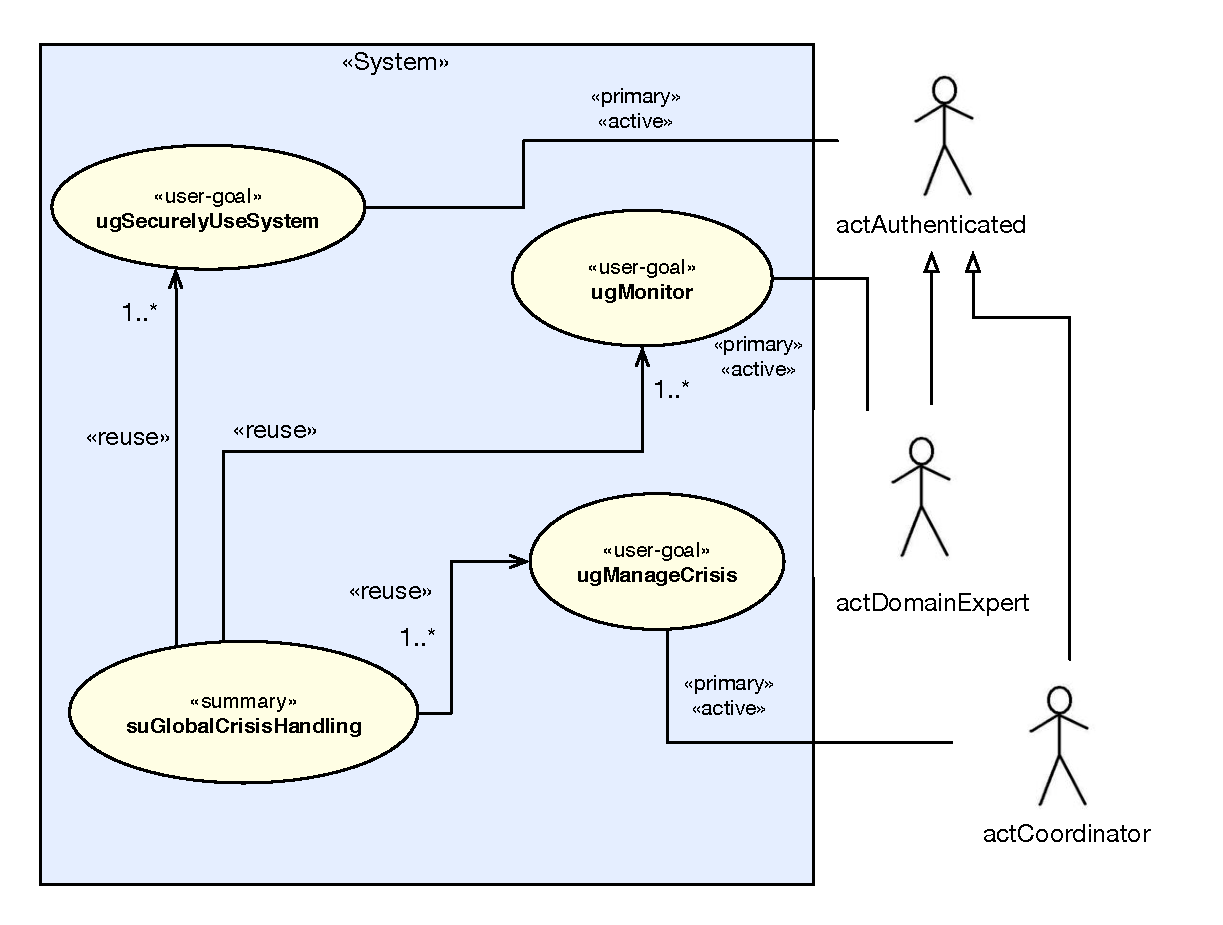
\includegraphics[width=180mm]{./images/ugGlobalCrisisHandling.eps}
 \normalsize}
 \end{center}
 \caption[\msricrash Use Case Diagram:  ugGlobalCrisisHandling Diagram]{\msricrash Use Case Diagram:  ugGlobalCrisisHandling}
 \label{fig:icrash-RE-UCD- ugGlobalCrisisHandling}
 \end{figure}
 \vspace{0.5cm}
